\vspace{-10mm}
\section{Experiments}\vspace{-2mm}
\label{sec:experiments}
In the following we briefly describe our experiment for visualizing the real large tractography for the validation of the proposed approach. The evaluation based on split factor and one heuristic trick to improve the visualization result are also presented.

\vspace{-2mm}
\subsection{dMRI and tractography segmentation}\vspace{-1mm}
%Diffusion MRI (dMRI) data allow to reconstruct the $3D$ pathways of axons within the white matter of the brain as a set of streamlines, called tractography. A streamline is a vectorial representation of thousands of neuronal axons expressing structural connectivity. 
Let the polyline $s =\{ \vec{x_1},\ldots,\vec{x}_{n_s}\}$, where $\vec{x} \in \mathbb{R}^3$, be a \emph{streamline} reconstructed from dMRI data by deterministic tractography algorithms~\cite{mori2002fiber}. 
Let the \emph{tractography} $ \mathbb{T}  = \{s_1,\ldots,s_N\}$ be defined as a set of $N$ streamlines. % reconstructed from dMRI data by deterministic tractography algorithms~\cite{mori2002fiber}. %, for which $N \sim 3 \times 10^5$ usually. 
%Recently, reconstruction and tracking algorithms~\cite{mori2002fiber,zhang2008identifying} allow to reconstruct the tractography from dMRI data. 
Our experiment is motivated by a clinical research hypothesis about the characterisation of the amiotrophic (ALS) disease, which is known to be affected by the corticospinal tract (CST)~\cite{cosottini2010evaluation,sage2009quantitative}. The first task is to segment the CTS from the full brain tractography $\mathbb{T}$. 

% Let $d:\mathcal{X} \times \mathcal{X} \mapsto \mathbb{R}^+$ be a distance function between streamlines. A common distance between streamlines is the symmetric minimum average distance (see~\cite{zhang2008identifying}) defined as $d(X_a,X_b) = \frac{1}{2}(\delta(X_a,X_b) + \delta(X_b,X_a))$ where \begin{equation}
%\label{equ:mam_distance}
%  \delta(X_a,X_b) = \frac{1}{|X_a|} \sum_{\mathbf{x}_i \in X_a}
%    \min_{\mathbf{y} \in X_b} ||\mathbf{x}_i - \mathbf{y}||_2.
%\end{equation}
In spite that recently there is an increasing literature in automatic
tractography segmentation using machine learning techniques~\cite{wang2011tractography,olivetti2011supervised}, applications in the clinical domain rely on manual segmentation. The manual segmentation process consumes a lot of time and effort due to the large number of streamlines, in the order of $3 \times 10^5$, which make it intrinsically difficult both to inspect and to unfold the anatomical structures. Moreover, 
%a lengthy and complex task for two reasons: first the tractography is a very large set of reconstructed neuronal pathways, 
%(see Figure~\ref{fig}). Second, 
it is claimed that there is a lack of software tools to support and to simply this segmentation process~\cite{olivetti2013fast}. In this experiment, we conceive a novel computer-assisted interactive process based on the method of multiple scales for representation the large tractography described in Section~\ref{sec:methods}. After computing the set of multiple scales $\mathsf{\textit{B}} = \{b_1, b_2, \ldots, b_k\}$, our tool first displays $\mathbb{T}$ as the cut at $b_1$, $\mathfrak{L}(b_1)$
%, which is a partition $\mathbb{T}$
; and let user select some of clusters to identify a superset of the streamlines of interest. This superset is then to be displayed at the next scale and again the user is requested to select the relevant clusters. The process of re-display and manual selection is iterated until the remaining streamlines faithfully represent the desired anatomical structure of interest.

%\paragraph*{ALS dataset:}
\vspace{0.55mm}
\textit{ALS dataset:}
the data we used in this experiment is recorded with a $3T$ scanner at Utah Brain Institute. It
consisted the recordings of $12$ ALS patients and $12$ healthy
controls; $64$ ($+1$, i.e. $b=0$) gradients; $b$-value$=1000$;
anatomical scan ($2 \times 2 \times 2mm^3$).  We reconstruct the
streamlines using EuDX, a deterministic tracking algorithm
~\cite{garyfallidis2012towards} from the DiPy
library~\footnote{\url{http://www.dipy.org}}. % We just present results on one subject.

%\paragraph*{Dissimilarity representation: }
\vspace{0.55mm}
\textit{Dissimilarity representation: }
due to the fact that 
%most of the state-of-the-art learning techniques often require the data to lie in a vectorial space, which is not the case of streamlines, which 
each streamline has different length and different number of points
%. And for this reason they cannot be directly represented in a common vectorial. In this case, 
we need to find a representation $\phi$ of streamline in a vectorial space, by mapping a streamline $s$ from its original space $\mathbb{T}$ to a vector of $\mathbb{R}^d$ - $\phi : \mathbb{T} \mapsto \mathbb{R}^d$, where $d$ is the dimension of the new space. One suggestion for this is the \emph{dissimilarity representation}~\cite{pekalska2002generalized}. It is a lossy Euclidean embedding algorithm was previously proposed
in~\cite{olivetti2012approximation} for streamlines. The dissimilarity representation
is defined as $\phi_{\Pi}^d(X):\mathcal{X} \mapsto \mathbb{R}^p$ s.t. $\phi_{\Pi}^d(X) = [d(X,\tilde{X}_1) ,\ldots, d(X,\tilde{X}_p)]$, 
%\begin{equation}
%  \phi_{\Pi}^d(X) = [d(X,\tilde{X}_1) ,\ldots, d(X,\tilde{X}_p)]
%\label{equ:dissimilarity_representation}
%\end{equation}
where $d$ is a distance function between streamlines, and $\Pi =
\{\tilde{X}_1, \ldots, \tilde{X}_p\} \subset \mathcal{X}$ is a set of
$p$ streamlines called \emph{prototypes}. %The quality of the Euclidean embedding is strongly dependent on the selection of the prototypes (see~\cite{pekalska2006prototype,olivetti2012approximation}).
More detail can be found in~\cite{olivetti2012approximation,pekalska2006prototype}.

\vspace{0.75mm}
%\noindent
By applying the hierarchical clustering algorithm (section~\ref{subsec:hierarchical}) on the dissimilarity approximation, the hierarchical tree $\mathcal{H}$ of the tractography $\mathbb{T}$ could be created.
\vspace{-2.75mm}
\subsection{Multiple scales for representation}\vspace{-1mm}
%\paragraph{\hspace{6mm}Scale measurement: }
As the measurement for computing the level of detail of a cluster $s(C_i)$, we use the height of the cluster $C_i$ within the hierarchical tree $\mathcal{H}$. The reason is that this measurement leads to continuous and thus provides smooth transitions on our hierarchical display. 
%Choosing the height of cluster as the measurement for the level of detail, together with a proper interactive tool to support roll up (down) operations, the visualization can be explored at different levels of abstraction easily.
 
Let $h$ be the height of hierarchical tree $\mathcal{H}$: $h = height(\mathcal{H})$, at the leaf $C_{leaf}$ of $\mathcal{H}$, the heigh is in the order of zero, thus $s_{min} = 0$. In the similar way, $s_{max} = 1$ because at the root $C_{root}$ of the tree $\mathcal{H}$, $heigh(C_{root}) = h$.  The range scale of $\mathcal{H}$ is $[s_{min}, s_{max}] = [0,1]$, and $\forall C_i \in \mathcal{H}, s(C_i) = \frac{height(C_i)}{h}$, where $heigh(C_i)$ is the heigh of the cluster $C_i$~\cite{yang2003interactive}. Intuitively, this measurement satisfies the condition of Definition~\ref{def:level_detail} about the level of detail in, because if $C_i$ is an ancestor of $C_j$, then $heigh(C_i) \geq heigh(C_j)$ and thus, $s(C_i) \geq s(C_j)$
%s = [0,1], where 0 is the whole leaves (streamlines) and 1 is the only one root. Scale s can be defined based on the height of tree h: 0/h, 1/h, ..., (h-1)/h, h/h; or the maximum distance of each node of the tree \cite{yang2003interactive}
%\paragraph{Choosing multiple scales for representation}

\vspace{0.5mm}
By looking at the local maxima of the goodness score as definition in~\ref{def:goodness_scale}, we can estimate the most relevant scale factors for representing the tree $\mathcal{H}$, and thus getting the multiple scale representation $\mathsf{\textit{B}} = \{b_1, b_2, \ldots, b_k\}$. The figure~\ref{fig:goodness_score} shows the plot lines of two goodness scores of subject $109$(left) and control $205$(right) from ALS dataset. 
%Focusing on the local maxima value of goodness score leads us to the meaningful scale factors for representing the tree $\mathcal{H}$. 
For example with subject $109$ (left) the multiple scale representation $\mathsf{\textit{B}}_{1}$ could be concluded as $\mathsf{\textit{B}}_{1} = \{\frac{8}{h_1}, \frac{10}{h_1}, \frac{12}{h_1}, \frac{18}{h_1}, \frac{22}{h_1},\frac{25}{h_1},\frac{27}{h_1}\}$, where $h_1$ is the heigh of the hierarchical tree$\mathcal{H}_{109}$ of subject $109$: $h_1= height(\mathcal{H}_{109})$. Similarly, with control $205$, $\mathsf{\textit{B}}_{2} = \{\frac{10}{h_2}, \frac{16}{h_2}, \frac{19}{h_2}, \frac{24}{h_2},\frac{27}{h_2}\}$, where $h_2= height(\mathcal{H}_{205})$. Taking into account that $b_i$ should be chosen from the small scale factor to the large one in order to satisfy the condition of an ordered set in the Definition~\ref{def:multi_scales_representation}, of which the underlying idea is to make sure a continuous and smooth order of visualization when users switch among these levels. This experiment exams the ability of our proposed method to compute the multiple scales representation for a large data. Note that we just present here the two samples of results, we also run on other subjects and get the equivalent multiple scale representation for each of them.
\begin{figure}
  \centering
  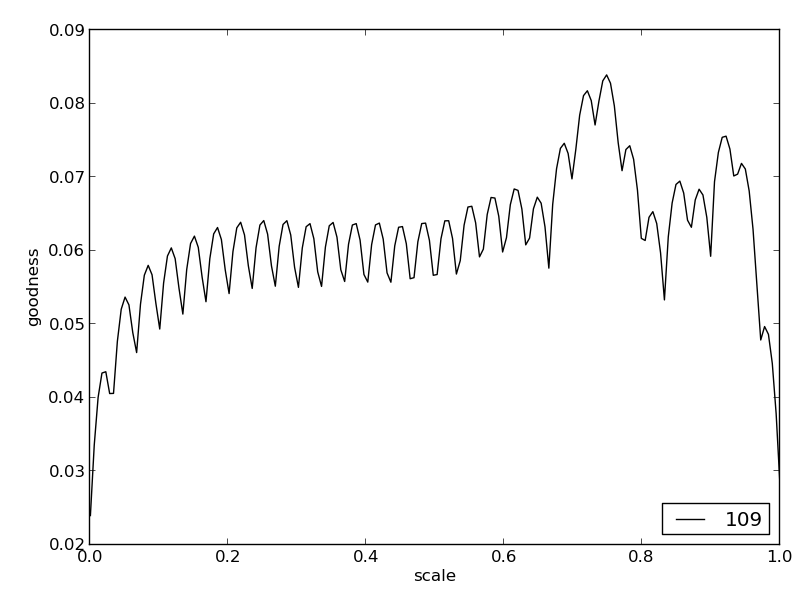
\includegraphics[width=6.6cm]{109_goodness_R_function.png}
  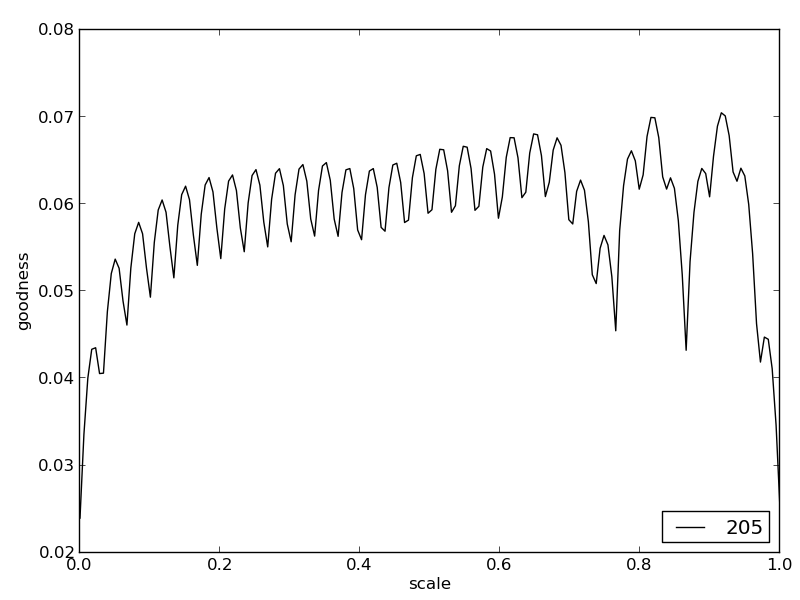
\includegraphics[width=6.6cm]{205_goodness_R_function.png}
  \caption{Goodness score of subject 109 and 205 from ALS dataset}% at different scale factor}
  \label{fig:goodness_score}
\end{figure}

%\paragraph*{Evaluate the multi scale representation}
\vspace{-4mm}We are now in the state of being ready to evaluate the multiple scale representation $\mathsf{\textit{B}} = \{b_1, b_2, \ldots, b_k\}$. Based on the Definition~\ref{def:best_scales} about the goodness of a scale factor $b \in \mathsf{\textit{B}}$, we implemented a program as the pseudo code in~\ref{alg:evaluate} with $\lambda_1 = 50$ and $\lambda_2=15$. In figure~\ref{fig:goodness_score} - left, we plot the mean goodness score of each multiple scale representation for subject 109 and control 205 from ALS dataset, together the standard derivation for $20$ iterations. Note that on the horizontal axis, the cut scales $l$ represented on the figure is the index of the corresponding real scale $\frac{l}{h}$. 
\begin{figure}
  \centering
  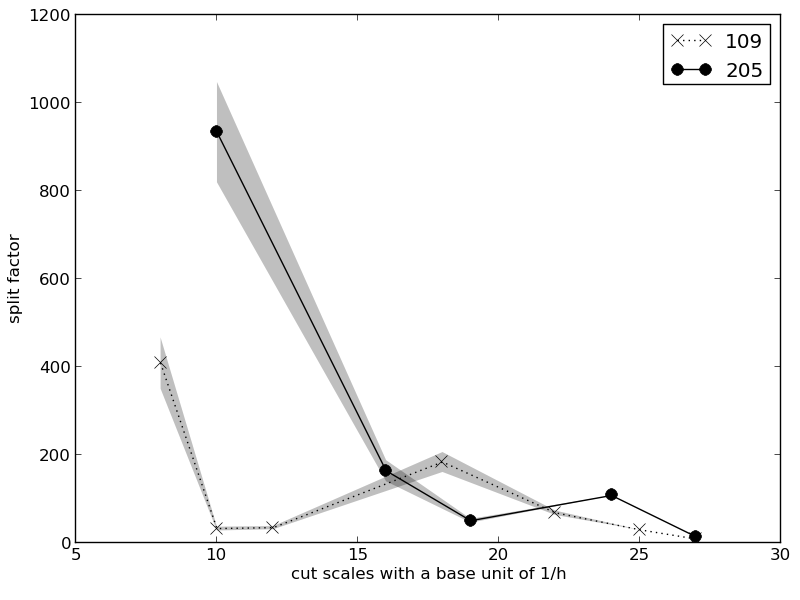
\includegraphics[width=6.6cm]{evaluate_cut_based_on_split_factor_130613_109_205_original.png}
  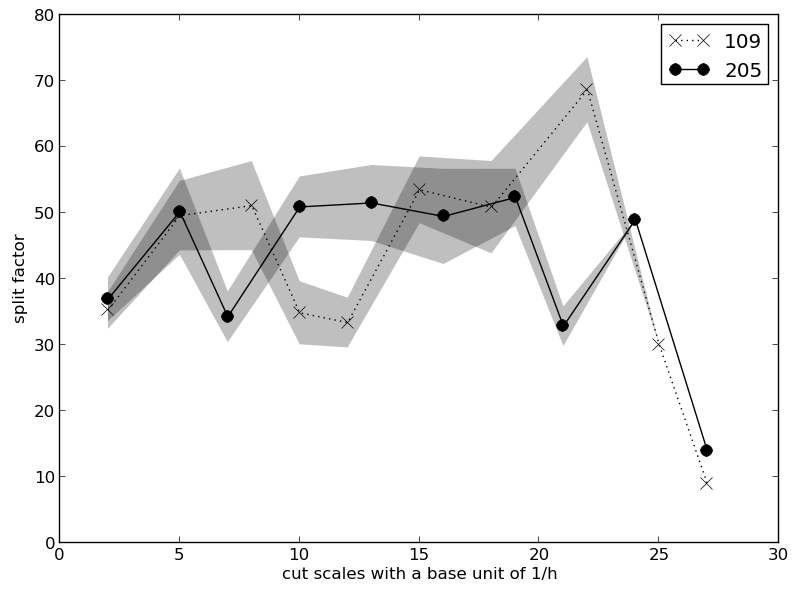
\includegraphics[width=6.6cm]{evaluate_cut_based_on_split_factor_130613_109_205.png}
  \caption{Split factor before(left) and after(right) adding heuristic constrains}
  \label{fig:split_factor}
\end{figure}

%\paragraph*{Heuristic for improving the multi scale representation}
\vspace{-0mm}Exept for the first chosen scale $b_1$, almost other scale $b_k \in \mathsf{\textit{B}}, k \neq 1$, the split factor $\xi(S_{(b_i,\lambda_2)},b_{i+1})$ satisfies the condition in Equation~\ref{equ:best_scale}. Note that from the leaf (scale $0$) the goodness score increases linearly, reaches the peak at scale $B_1$, and then gets a fluctuating variety. It shows that the split factor of the cut at $b_1$ to the leaf (scale $0$), $\xi(S_{(b_1,\lambda_2)},0))$, is usually very large comparing with other split factors. However, in the point view of visualization, all the split factor $\xi(S_{(b_i,\lambda_2)},b_{i+1})$ should be around $\lambda_1$. Due to this, 
%for the saking of better representation, 
we add an heuristic constrain to the chosen scale set: the distance between 
%two closest chosen scale
$b_i$ and $b_{i-1}$ should not exceed a threshold $\delta$: $d(b_i,b_{i-1}) \leq \delta$ (in the case of $b_1$, the distance with the leaf, $d(b_1,0)$, is used). The results after adding constrain are showed in the figure~\ref{fig:goodness_score} - right (with $\delta = 4/h$) where the mean split factor is close to $\lambda_1 = 50$. This approach is run on many subjects from ALS dataset, the sizes of which vary from $200K$ to $300K$. These results demonstrate that our proposed method of choosing multiple scales for visualization large data is efficient and robust to the size of the large data. 


